\section{\DYNAMICO is}

\DYNAMICO \footnotemark is a new dynamical core for LMD-Z, the atromspheric GCM part
of IPSL-CM Earth System Model.
%
\DYNAMICO is funded by the Indo-French Centre for the Promotion of
Advanced Research, by IPSL and by the G8 Research Councils Initiative on
Multilateral Research Funding, project ICOMEX.


\footnotetext{
This section is based on the \DYNAMICO Wiki page (\url{http://forge.ipsl.fr/dynamico/wiki})
}



The primary goal of \DYNAMICO is to re-formulate in LMD-Z the horizontal
advection and dynamics on a icosahedral grid, while preserving or
improving their qualities with respect to accuracy, conservation laws
and wave dispersion.
%
A broader goal is to revisit all fundamental features of the dynamical
core, especially the shallow-atmosphere/traditional approximation, the
vertical coordinate and the coupling with physics.
%
Also efficient implementation of present and future supercomputing
architectures is a key issue.

This manual describes the overview of \DYNAMICO and each kernel program
briefly.
%
For the details of \DYNAMICO, see
\cite{gmd-8-3131-2015},
etc.


Kernel programs for \DYNAMICO are taken from \DYNAMICO ver 1.0, r339.
%
Main feature of \DYNAMICO-1.0 are;
\begin{itemize}
 \item hydrostatic, traditional shallow atmosphere,
 \item icosahedral-hexagonal C-grid in horizontal, mass-based Lorentz
       staggering in vertical,
 \item Mimetic finite difference + slope-limited finite volume
       transport, and
 \item explicit Runge-Kutta time stepping.
\end{itemize}



\section{Governing equations}

Basic scheme of \DYNAMICO is the energy/voticity conserving schemes and
the curl (vector-invariant) form.
%
To deliver governing equations, \DYNAMICO adopts the Hamiltonian
formulation of the equations of motion.
%
This Hamiltonian theory has been extended for compressible hydrostatic
flows and for non-Eulerian vertical coordinates \citep{JAS-D-13-0339,MWR-D-14-00069}.
%
Derivation of governing equations is complicated, we skip it here. See
\cite{gmd-8-3131-2015} etc.




\section{Horizontal and vertical grid}

\DYNAMICO adopts the icosahedral-hexagonal C-grid in horizontal and
mass-based Lorentz staggering grid in vertical.
%
\autoref{f:ico_c_grid} shows horizontal and vertical grids.

Scalar variables, such as entropy $\Theta$, are defined on the center of
hexagonal control volume (circle points in the figure), velocities and fluxes,
are defined on the edge (square points), and tracer are
defined on the vertex (triangle points).
%
See \cite{gmd-8-3131-2015} for details.


\begin{figure}
 \centering
 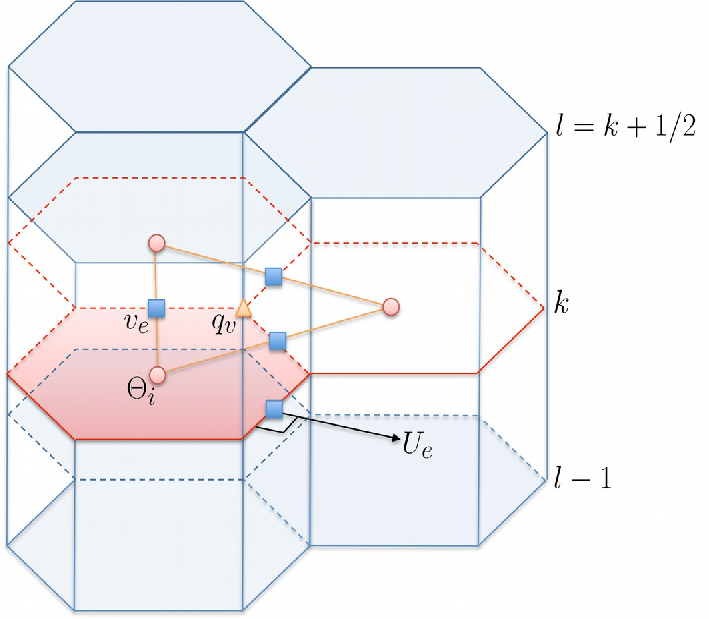
\includegraphics[scale=1]{figs/AIMES_DYNAMICO-08-0.png}
 \caption{Icosahedral C-grid and Lorenz grid.}\label{f:ico_c_grid}
%http://www.lmd.polytechnique.fr/~dubos/Talks/2014DubosAGU.pdf
\end{figure}



\section{Parallelization}

Like \NICAM and \DYNAMICO, icosahedral grids on entire globe can be
separated by 10 ``diamonds'', each are consist of neighboring two
triangles of an icosahedron.
%
Each diamonds can be divided in \src{nsplit_i}$\times$\src{nsplit_j} areas,
and one of divided area,
called ``patch'' in \DYNAMICO, is the basis of domain decomposition.
%
\src{nsplit_i} and \src{nsplit_j} are control parameter and read from
configuration file on execution.
%
One MPI process can handle \src{ndomain} patches, which is decided by
the number of total patchs and the number of MPI processes.



\section{Data structure}\label{s:data_structure}

Basic data structure in \DYNAMICO is a \src{t_field}, as shown in
\autoref{l:t_field}.
%
One instance of \src{t_field} is to access one field within one patch.
%
One MPI process may handle several patches, and one field may be usually
an array of \src{t_field}.
%
Allocation and halo-exchange routines are work on \src{t_field(:)}
variables, and other high-level computational routines work on them, too.
%
See the next section as an example.

\begin{LstF90}[%
caption={\src{t_field} structure},%
label={l:t_field}%
]
  TYPE t_field
    CHARACTER(30)      :: name
    REAL(rstd),POINTER :: rval2d(:)
    REAL(rstd),POINTER :: rval3d(:,:)
    REAL(rstd),POINTER :: rval4d(:,:,:)

    INTEGER,POINTER :: ival2d(:)
    INTEGER,POINTER :: ival3d(:,:)
    INTEGER,POINTER :: ival4d(:,:,:)

    LOGICAL,POINTER :: lval2d(:)
    LOGICAL,POINTER :: lval3d(:,:)
    LOGICAL,POINTER :: lval4d(:,:,:)

    INTEGER :: ndim
    INTEGER :: field_type
    INTEGER :: data_type
    INTEGER :: dim3
    INTEGER :: dim4
  END TYPE t_field
\end{LstF90}

One of members of \src{t_field} are pointer to the array of
\src{REAL(rstd)}, \src{INTEGER} or \src{LOGICAL}, and whose dimension is
one, two or three.
%
If the field is horizontal, such as surface pressure or sea surface
temperature, \src{rval2d} is used.
%
Note that horizontal index $I$ and $J$ are merged to one dimension.


\autoref{f:aimes_dynamico-30-0} shows horizontal indexing in \DYNAMICO.
%
As shown in previous chapter, \DYNAMICO adopts icosahedral grid, and
control volume is hexagonal as usual.
%
One ``patch'' is rhomboid, and can be indexed as two-dimensional, each
size are \src{iim} and \src{jjm}, as shown in left figure of
\autoref{f:aimes_dynamico-30-0}.
%
These can be re-written as usual orthogonal i-j plane, shown in the
right figure of \autoref{f:aimes_dynamico-30-0}.
%
The \src{n} point in the figure is surrounded by
six neighbouring cells, named \src{right}, \src{rup}, etc.
%
So stencil calculation comes from finite difference in horizontal uses
seven points, not five as in usual orthogonal grid.

\begin{figure}[htpb]
\centering
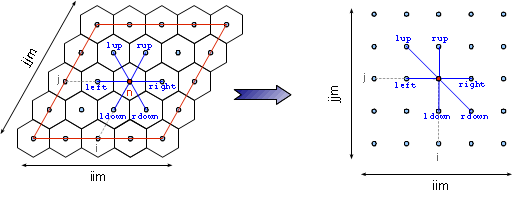
\includegraphics[scale=0.7]{figs/AIMES_DYNAMICO-30-0.png}
\caption{Horizontal indexing}\label{f:aimes_dynamico-30-0}
\end{figure}

The number of the edge point is three times larger than that of the center point.
As shown in \autoref{f:rel_center_edge}, each center point manages three edge points.
These points are named \src{u_right}, \src{u_lup}, and \src{u_ldown}.

\begin{figure}[htpb]
\centering
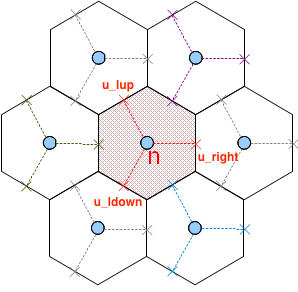
\includegraphics[scale=0.5]{figs/AIMES_DYNAMICO-30-1.png}
\caption{Relationship of center points and edge points}\label{f:rel_center_edge}
\end{figure}

To allocate one \src{t_field} instance, subroutine \src{allocate_field}
is called.
%
Below is the example of allocating orography named ``phis''.

\begin{LstF90}
 ! Time-independant orography
    CALL allocate_field(f_phis,field_t,type_real,name='phis')
\end{LstF90}



\section{Code structure}

Global program structure of \DYNAMICO is as follows.

In the main program, after the various initialization, time step loop is
carried by a single subroutine \src{timeloop}.
%
\autoref{f:pad_timeloop} shows PAD (Problem Analysis
Diagram)\footnotemark of main processes in subroutine \src{timeloop}.
%
As seen in the top of this PAD,

\footnotetext{See \autoref{s:pad} for reading PAD.}

\begin{figure}[htb]
 \centering
 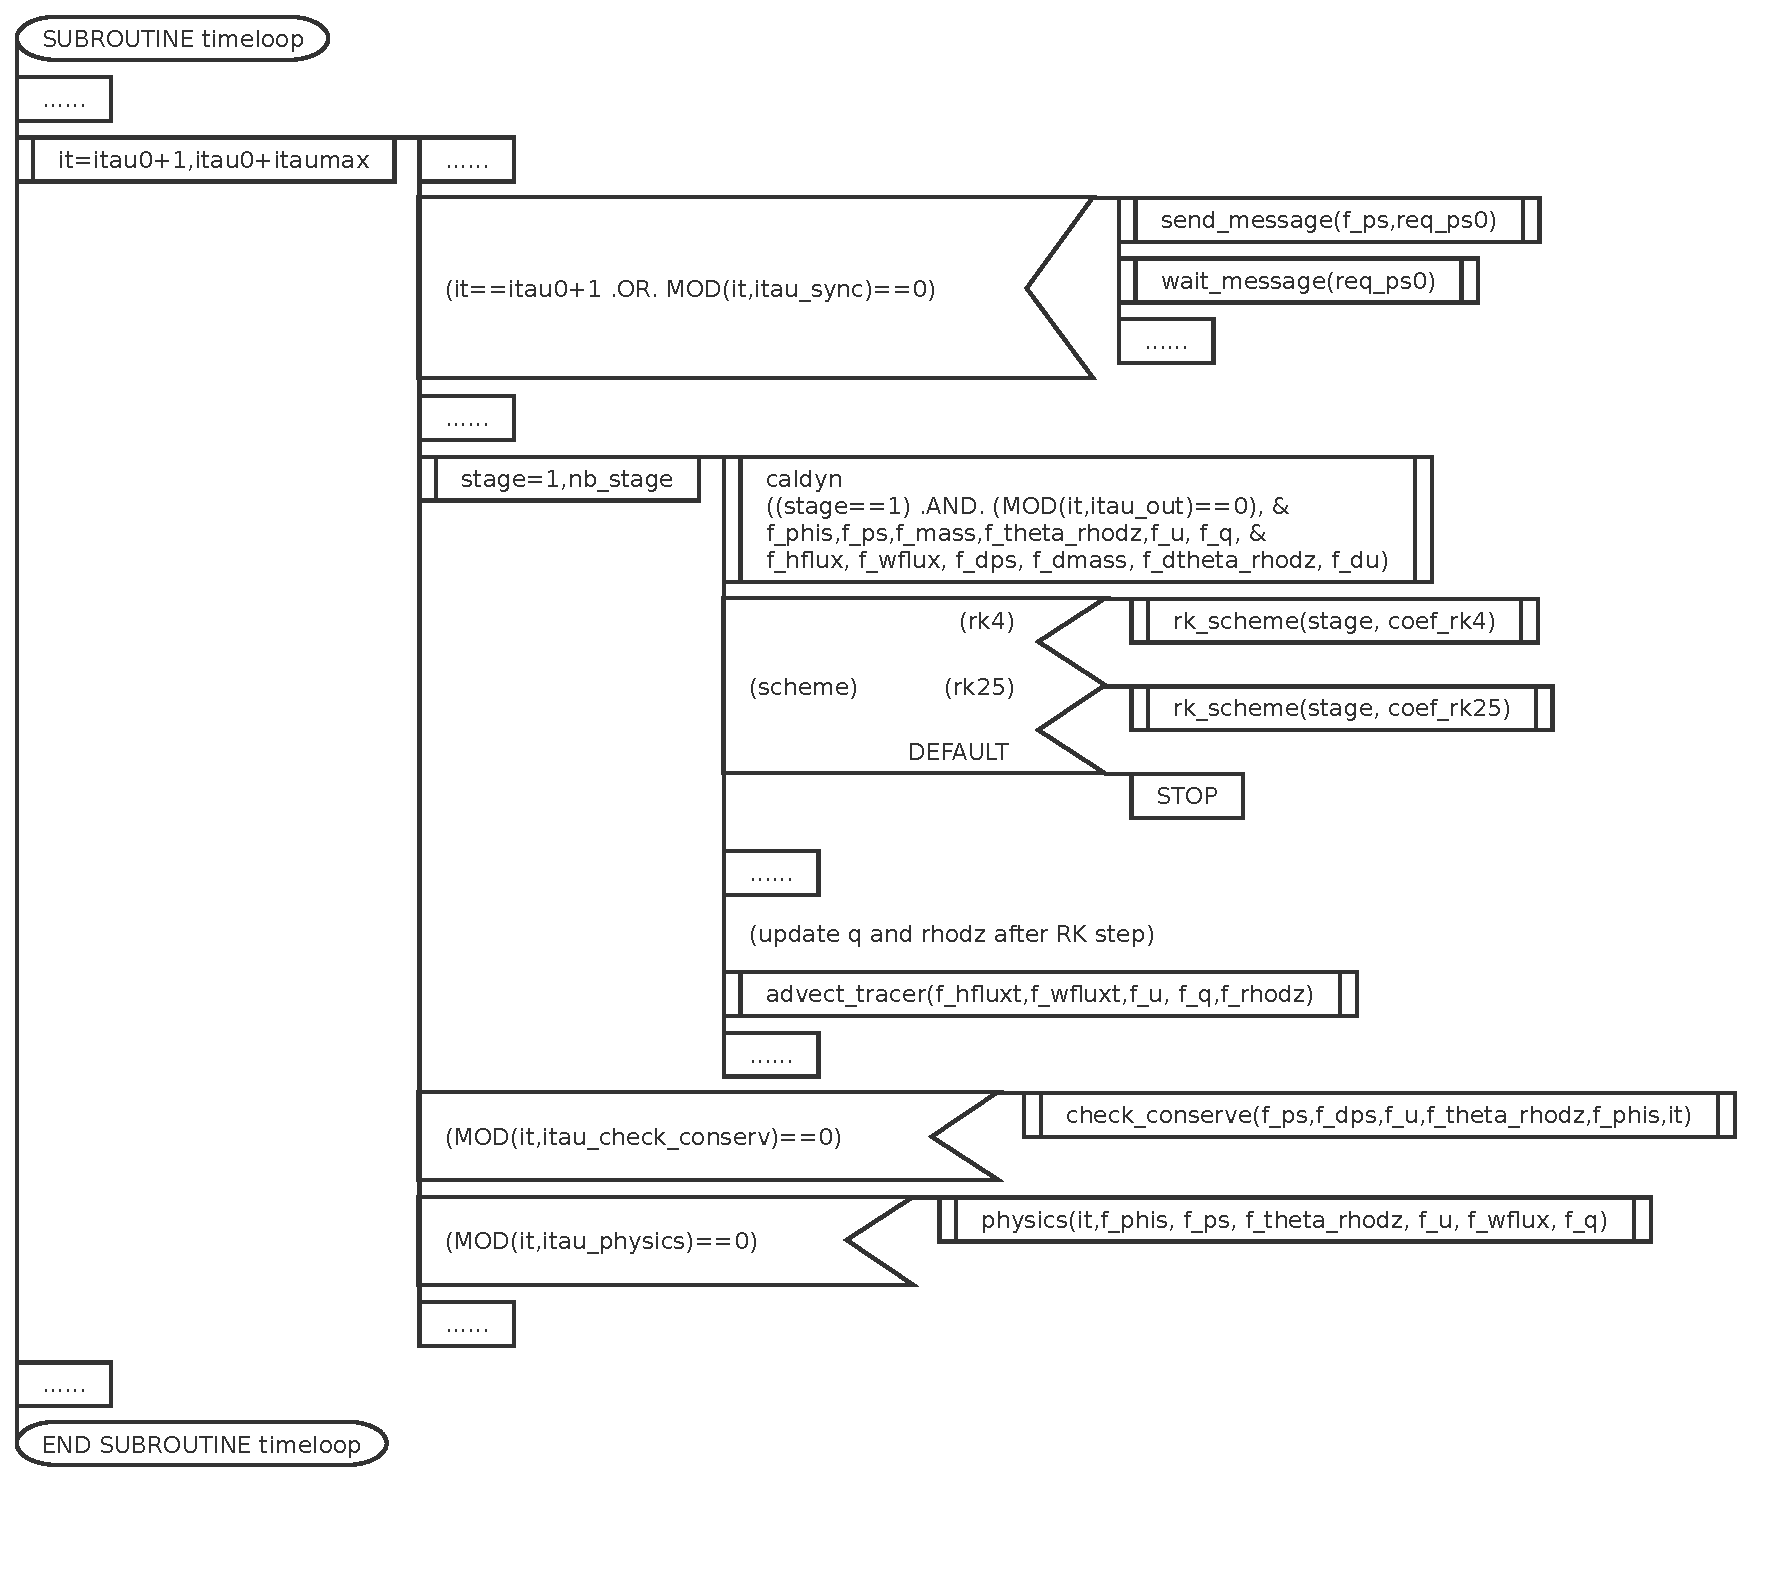
\includegraphics[scale=.4]{figs/timeloop.pdf}
 \caption{PAD of \src{timeloop}}\label{f:pad_timeloop}
\end{figure}

Main time step loop is described in first \src{it} loop, from step
\src{itau0} to \src{itau0+italmax}.
%
First IF block in this loop is for halo exchange of several fields,
using subroutine \src{send_message} and \src{wait_message}.
%
In the next \src{stage} loop subroutine \src{caldyn}, one of
\src{*_scheme} and \src{advect_tracer} are called sequentially.
%
Subroutine \src{caldyn} calculate dynamical terms such as potential
vorticity, etc.
%
Subroutine \src{*_scheme} is for time-advancing. For example,
\src{rk_scheme} uses Runge-Kutta scheme.
%
This is a default scheme for this kernel package.
%
Subroutine \src{advect_tracer} is to calculate advection of tracer
quantities.
%
Here variable \src{nb_stage} in the loop range is the number of
iteration necessary for each time-advancing scheme. For example,
\src{nb_stage=1} for Euler scheme, \src{nb_stage=4} for Runge-Kutta scheme.
%
Finally, if time step \src{it} is at \src{itau_physics}'th step,
subroutine \src{physics} is called to calculate physics part.



\autoref{l:definition_caldyn} is the definition part of subroutine
\src{caldyn}\footnotemark,
and \autoref{f:pad_caldyn} is the PAD of it.
%
\footnotetext{Here is the version in \file{caldyn_gcm.f90}}
%
Note that all of current four kernel program in this package is taken
from the subroutine called from this \src{caldyn} (See \autoref{s:kernelize}).
%
As mentioned in \autoref{s:data_structure}, all of fields used in this
subroutine is given as pointers of instance of \src{t_field}.

\begin{LstF90}[%
caption={Definition part of \src{caldyn}},%
label={l:definition_caldyn}%
]
  SUBROUTINE caldyn(write_out,f_phis, f_ps, f_mass, f_theta_rhodz, f_u, f_q, &
       f_hflux, f_wflux, f_dps, f_dmass, f_dtheta_rhodz, f_du)
    USE icosa
    USE disvert_mod, ONLY : caldyn_eta, eta_mass
    USE vorticity_mod
    USE kinetic_mod
    USE theta2theta_rhodz_mod
    USE wind_mod
    USE mpipara
    USE trace
    USE omp_para
    USE output_field_mod
    USE checksum_mod
    IMPLICIT NONE
    LOGICAL,INTENT(IN)    :: write_out
    TYPE(t_field),POINTER :: f_phis(:)
    TYPE(t_field),POINTER :: f_ps(:)
    TYPE(t_field),POINTER :: f_mass(:)
    TYPE(t_field),POINTER :: f_theta_rhodz(:)
    TYPE(t_field),POINTER :: f_u(:)
    TYPE(t_field),POINTER :: f_q(:)
    TYPE(t_field),POINTER :: f_hflux(:), f_wflux(:)
    TYPE(t_field),POINTER :: f_dps(:)
    TYPE(t_field),POINTER :: f_dmass(:)
    TYPE(t_field),POINTER :: f_dtheta_rhodz(:)
    TYPE(t_field),POINTER :: f_du(:)

    REAL(rstd),POINTER :: ps(:), dps(:)
    REAL(rstd),POINTER :: mass(:,:), theta_rhodz(:,:), dtheta_rhodz(:,:)
    REAL(rstd),POINTER :: u(:,:), du(:,:), hflux(:,:), wflux(:,:)
    REAL(rstd),POINTER :: qu(:,:)
    REAL(rstd),POINTER :: qv(:,:)

! temporary shared variable
    REAL(rstd),POINTER  :: theta(:,:)
    REAL(rstd),POINTER  :: pk(:,:)
    REAL(rstd),POINTER  :: geopot(:,:)
    REAL(rstd),POINTER  :: convm(:,:)
    REAL(rstd),POINTER  :: wwuu(:,:)

    INTEGER :: ind
    LOGICAL,SAVE :: first=.TRUE.
\end{LstF90}

\begin{figure}[htb]
\centering
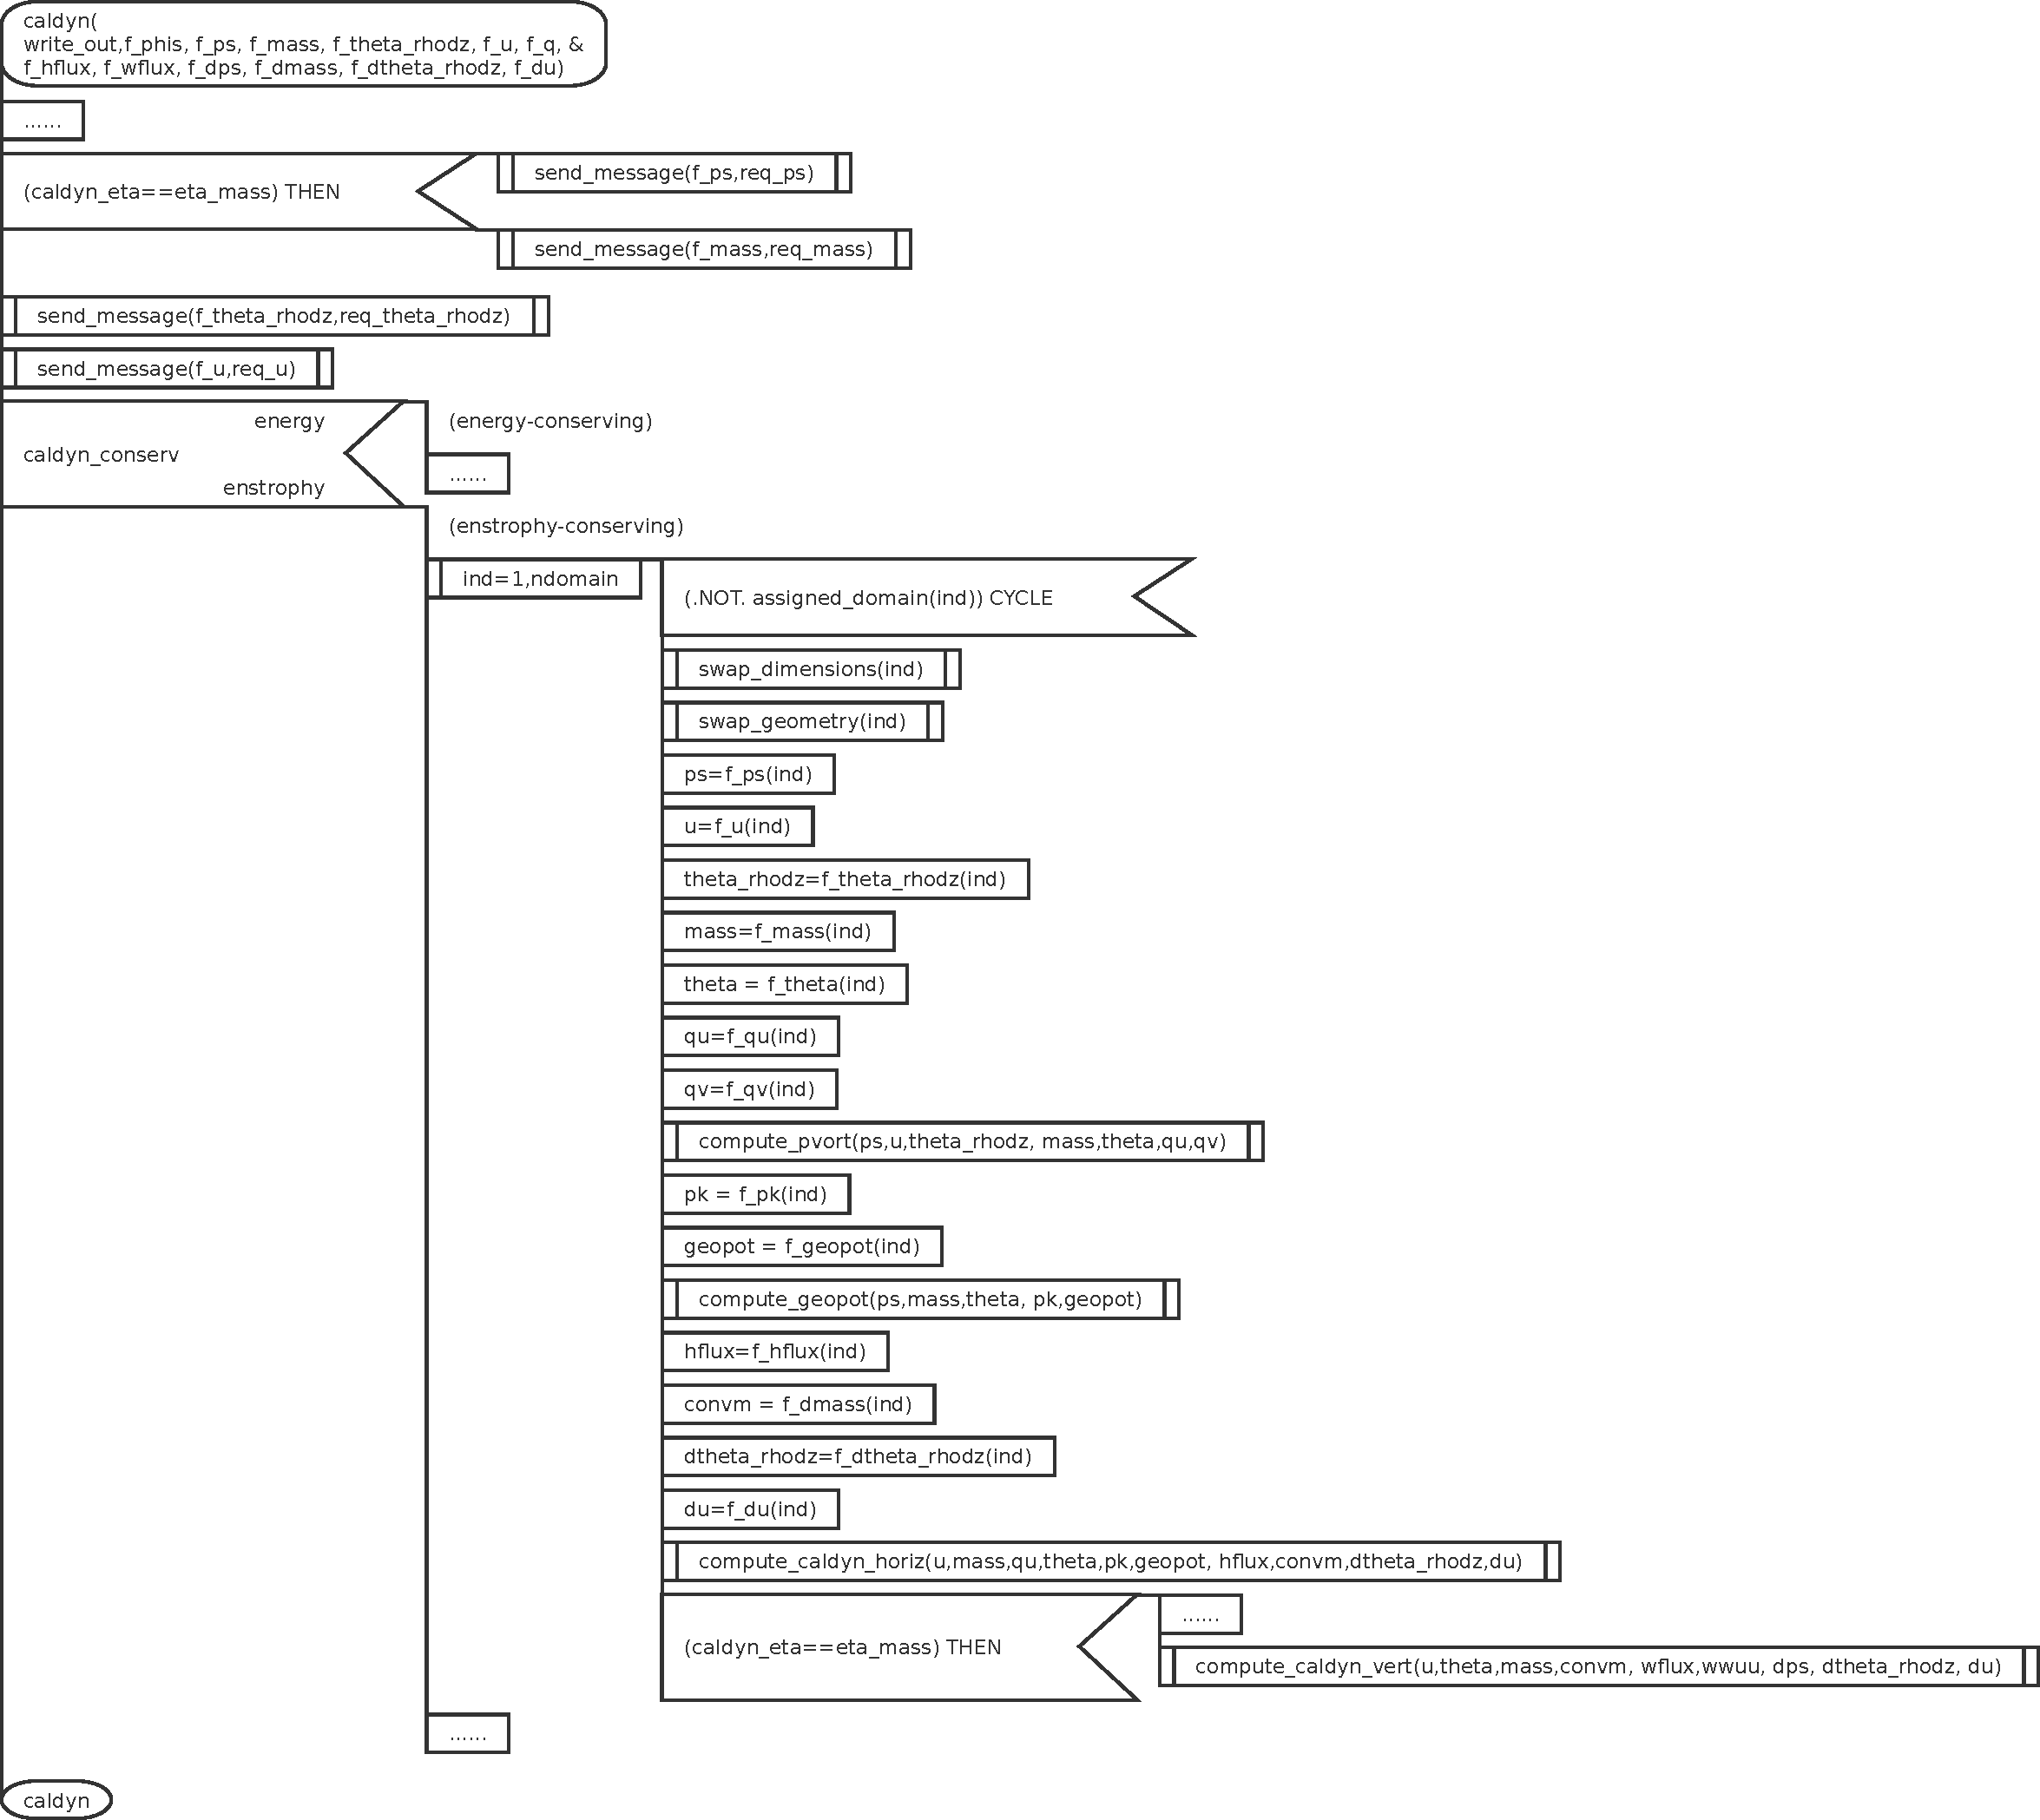
\includegraphics[scale=.4]{figs/caldyn.pdf}
\caption{PAD of \src{caldyn}}\label{f:pad_caldyn}%
\end{figure}

In \autoref{f:pad_caldyn} there are some assignment from
\src{t_field} to real pointer, such as \src{ps = f_ps(ind)}.
%
This is defined as module procedure and generic subroutine
\src{get_val} and using interface assignment.
%
All of them are defined in module \src{field_mod} in \file{field.f90}.

